\chapter{Results}
\label{ch:results}
\section{Univariate Model}
Using the grid search algorithm for automated model selection, each of the four stocks' returns yielded varying results. $\mathbf{Figure~5.1}$ shows the fitted model parameters for the two most optimal models, based on the minimization of the selected loss function: Akakie's Information Criterion (AIC). After the automated selection, I manually selected the model I would choose to implement based on significant parameters, model complexity, and residual distribution. As explained in $\mathbf{Section~4.3}$, there is more to a "best" model than the minimization of a loss function, so to ensure the best results I took a greater holistic approach to selection.

\subsection{Lloyd's}

The best models for Lloyds were \textbf{EGARCH(1,1), skewed-t}  \textbf{EGARCH(1,3),  skewed-t}. The two had negligible differences in AIC, but looking at the parameters, the added coefficients to the \textbf{(1,3)} model not only were insignificant, but it rendered the intercept and $\mathbf{\beta_1}$ coefficient insignificant as well (p-value $<$ 0.05). For this reason I chose the \textbf{EGARCH(1,1)} model, simpler and more significant parameters.

\subsection{Tesco}
The best models for Tesco were \textbf{EGARCH(1,2), students-t} and \textbf{EGARCH(2,1), students-t}. Model selection in this case was quite difficult, though the models themselves wouldn't produce overly different results. Both had 3 significant non-slope parameter, as well as the distribution parameter, while having insignificant intercepts. Because of the negligible difference in parameters, I defaulted to the automated model selection choice of  $\mathbf{EGARCH(1,2)~students-t}$ because of its minimum AIC value. 

\subsection{Rolls Royce}
The best models for Rolls Royce were \textbf{EGARCH(1,3), students-t} and \textbf{EGARCH(1,2), skewed-t}. The two had negligible differences in AIC, and no different in model coefficients (barring rounding error). The difference was the distribution of the residuals. To make a decision on which model, I fit using Maximum Likelihood Estimation the residuals to a distribution and found that again there was negligible difference. I chose the $\mathbf{EGARCH(1,3),~ students-t}$ model because it had the minimum AIC.  

\subsection{Vodafone}
The best models for Vodafone were \textbf{EGARCH(3,1), students-t} and \textbf{EGARCH(1,2), students-t}. The two had negligible differences in AIC, but looking at the parameters, the added coefficient to the (1,3) was not significant $\alpha_3$ and neither was $\omega$ the intercept. For this reason I chose the $\mathbf{EGARCH(1,2),~students-t}$ model, simpler and more significant parameters.  

\begin{figure}[hbt!]
\begin{subfigure}{.49\linewidth}
  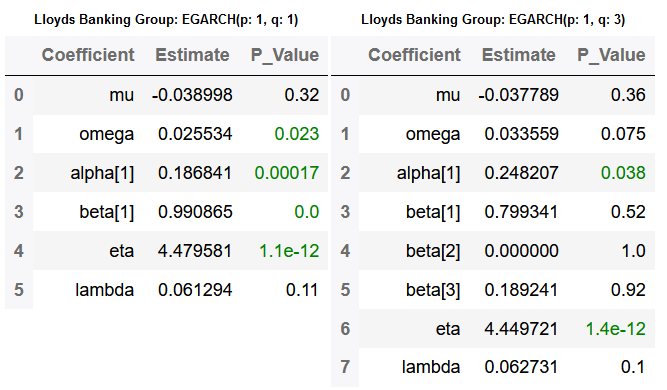
\includegraphics[width=\linewidth]{images/parameters/Lloy.png}
  \caption{LLOY}
  \label{fig:A}
\end{subfigure} % <-- "\hfill"
\begin{subfigure}{.49\linewidth}
  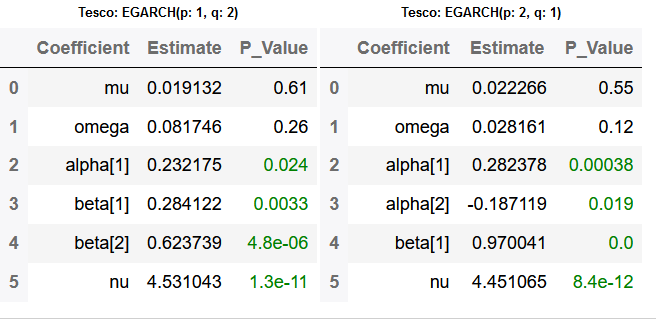
\includegraphics[width=\linewidth]{images/parameters/tesco.png}
  \caption{TSCO}
  \label{fig:B}
\end{subfigure}
\medskip % create some *vertical* separation between the graphs
\begin{subfigure}{.49\linewidth}
  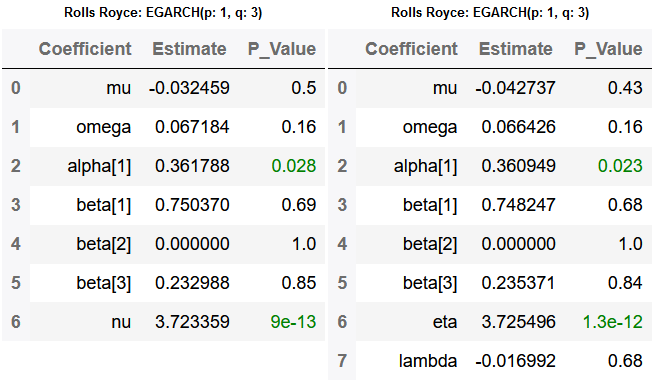
\includegraphics[width=\linewidth]{images/parameters/rr.png}
  \caption{RR}
  \label{fig:C}
\end{subfigure} % <-- "\hfill"
\begin{subfigure}{.49\linewidth}
  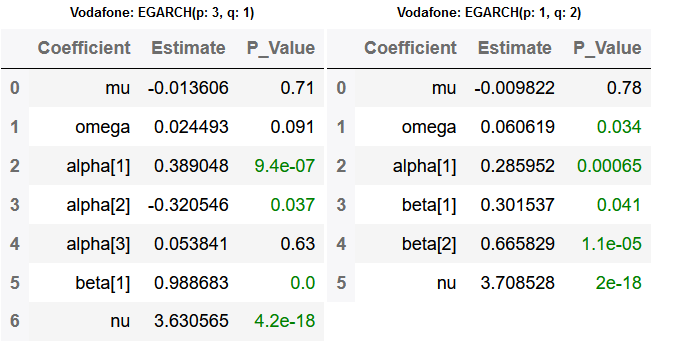
\includegraphics[width=\linewidth]{images/parameters/vod.png}
  \caption{VOD}
  \label{fig:D}
\end{subfigure}
\caption{Best Univariate Model Parameters}
\end{figure}

\subsection{Forecast Performance}
The resultant forecasts from these models yielded different results, and it became apparent that the fit and forecasts for Tesco and and Vodafone in both fixed and expanding window methodology were superior to that of Rolls Royce and Lloyd's. For the most accurate two models, the expanding window was more accurate than the fixed window. A great point of concern in the model fititng was the serious issues with the accuracy of the model for Rolls Royce returns, interestingly, the performance of the \textbf{EGARCH(1,3)} was worse than that of a model that simply took the mean of the information set's standard deviations. To interpret the table output, the scale of the chart was in \% so the best model, Vodafone, found itself within 2.21\% of the volatility proxy of squared centered returns on average. Though the models were simple, only including returns without any other information, a volatility forecast for 25 days with a mean absolute error of less than 2.4\% I believe to be very encouraging. For Tesco and Vodafone, the volatility forecasts are quite accurate and building complexity and information on top of these models could be quite advantageous. To continue work with Lloyd's and Rolls Royce, there is greater tuning to be done, these models are pretty much useless and should not be used moving forward.  
\begin{figure}[H]
\begin{subfigure}{.49\linewidth}
  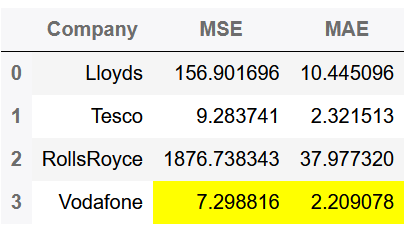
\includegraphics[width=\linewidth]{images/garchForecasts/expandingWindow.png}
  \caption{Expanding Window}
  \label{fig:A}
\end{subfigure} % <-- "\hfill"
\begin{subfigure}{.49\linewidth}
  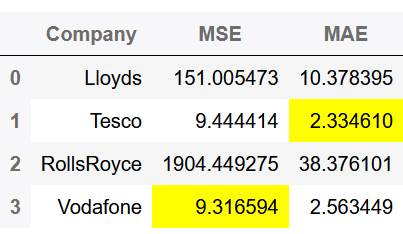
\includegraphics[width=\linewidth]{images/garchForecasts/fixedWindow.png}
  \caption{Fixed Window}
  \label{fig:B}
\end{subfigure}
\caption{Forecast Generalization Error}
\end{figure}

\section{Dynamic Conditional Correlation Model}
Implementing the DCC model on the model volatilities and the Irithmics conditional volatility did not immediately lead to a visualization or indication of any encouraging relationships between the Irithmics predicted short/sell probabilities and the stock returns. For the four stocks, the standard Pearson correlation coefficient between the two variables was about 0.07 - 0.09. Then using the dynamic model, I hoped to see if there were any events during the time series that there were significantly higher times of correlation, but unfortunately I never found this to be proven true. The highest correlated stock with Irithmics probabilities was Lloyd's, with its maximum conditional correlation was the beginning of February and June, but this value only reached 0.12. Ideally, this value would be much higher, as the next step in this analysis was to incorporate this value as an exogenous covariate implemented through linear regression. Theoretically all was not lost, as with financial applications any small fraction of increased accuracy can lead to large savings in a risk mitigation setting with investments, but greater correlation is obviously desired. To assist in the visualization over time, $\mathbf{Figure~5.3}$ plots the $\mathbf{EGARCH(1,1)}$ volatility with the Irithmics conditional volatility to show the linear relationship in a scatter plot and includes the sample correlation coefficient. Again, these results were not at all encouraging, but did not necessarily omit the prospect of slight increases in forecast accuracy by incorporating the exogenous data to the conditional volatility models \cite{DirtyQuant}. 


\begin{figure}[hbt!]
\begin{subfigure}{.49\linewidth}
  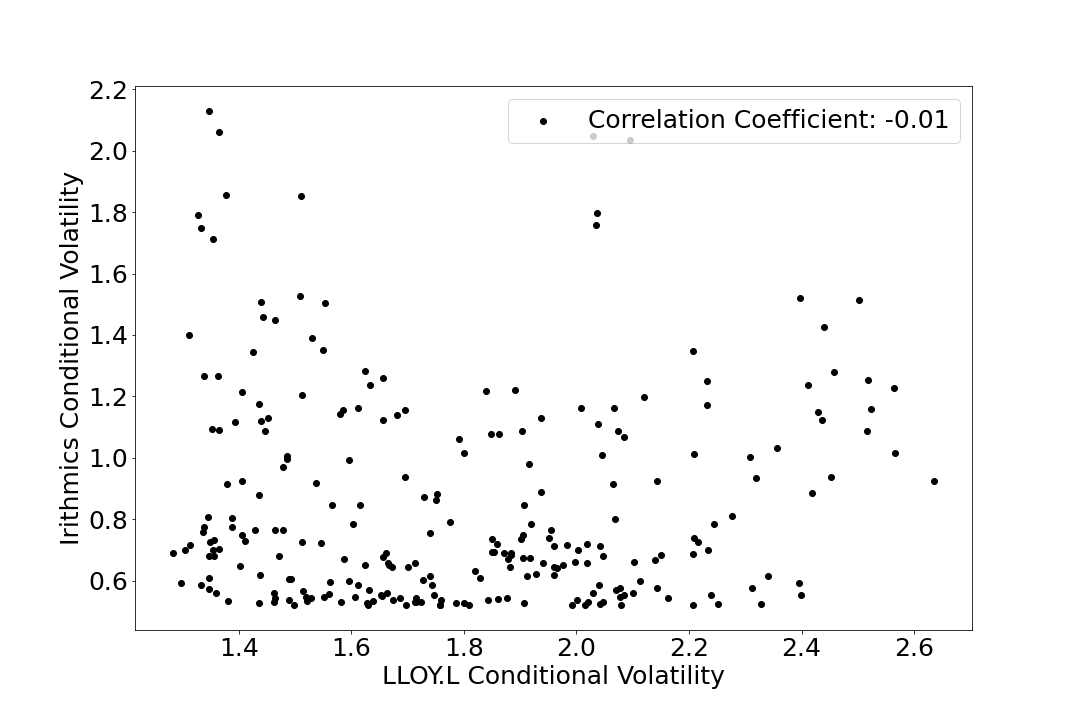
\includegraphics[width=\linewidth]{images/dcc_scatter/plot 1.png}
  \caption{LLOY}
  \label{fig:A}
\end{subfigure} % <-- "\hfill"
\begin{subfigure}{.49\linewidth}
  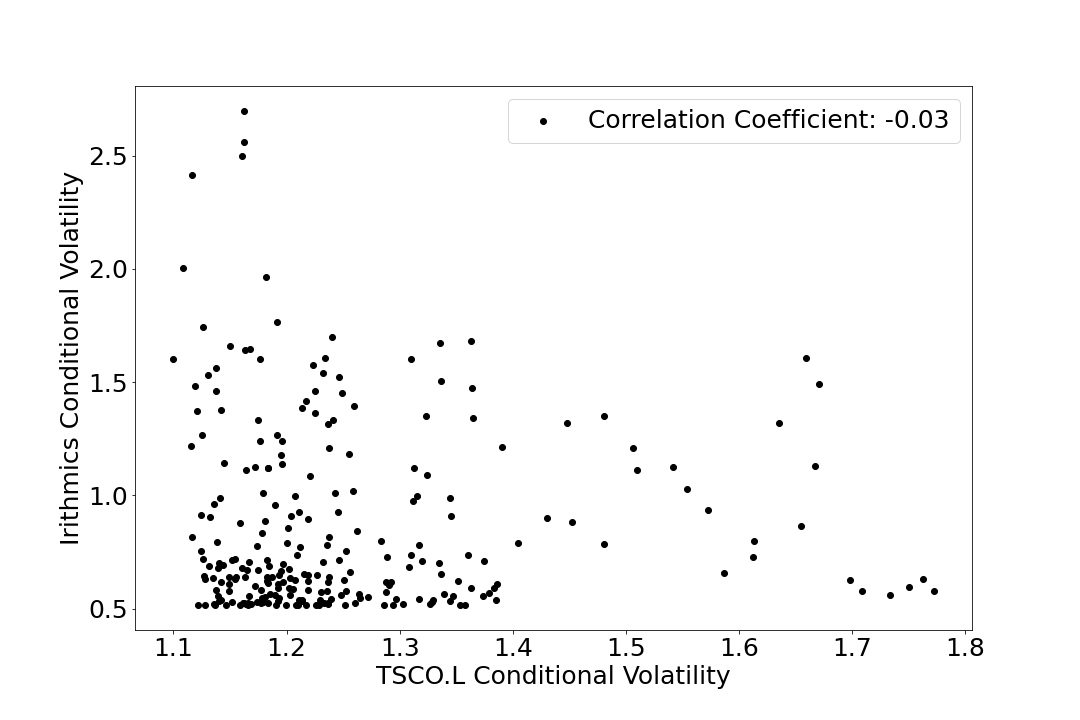
\includegraphics[width=\linewidth]{images/dcc_scatter/plot 2.png}
  \caption{TSCO}
  \label{fig:B}
\end{subfigure}
\medskip % create some *vertical* separation between the graphs
\begin{subfigure}{.49\linewidth}
  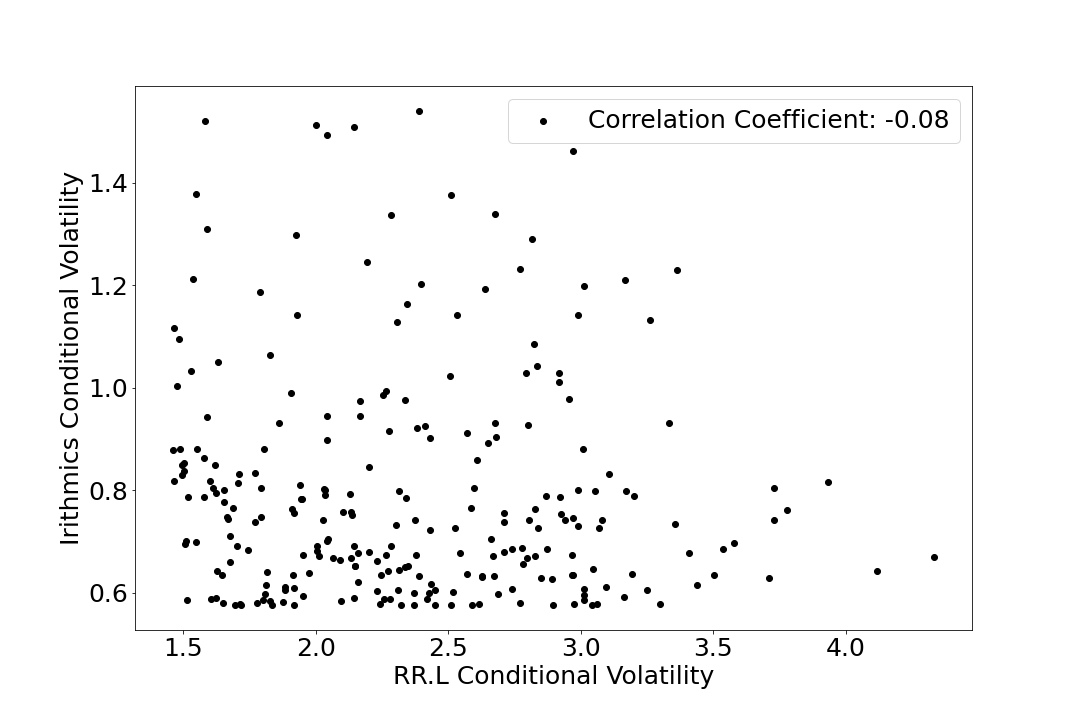
\includegraphics[width=\linewidth]{images/dcc_scatter/plot 3.png}
  \caption{RR}
  \label{fig:C}
\end{subfigure} % <-- "\hfill"
\begin{subfigure}{.49\linewidth}
  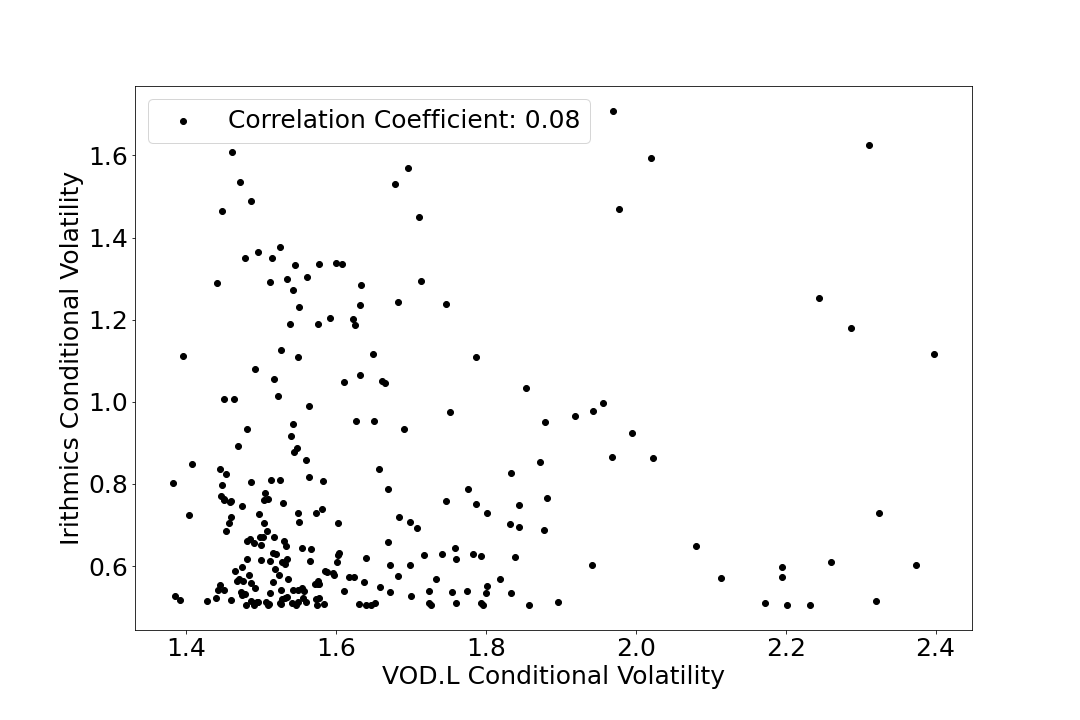
\includegraphics[width=\linewidth]{images/dcc_scatter/plot 4.png}
  \caption{VOD}
  \label{fig:D}
\end{subfigure}
\caption{DCC Scatter Plot}
\end{figure}

\section{Exogenous Covariate Model}
\subsection{Forecast Performance}
$\mathbf{Figure~5.4}$ highlights the comparative performance of the conditional volatility models forecasts with and without the exogenous covariate. 
\begin{figure}[H]
\centering
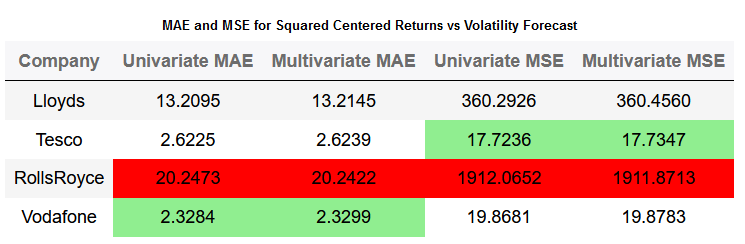
\includegraphics[scale=0.45]{images/multiGarch/GenErrorMSEMAE.png}
\caption{Multivariate Model Generalisation Error}
\label{fig: Multivariate Gen Error}
\end{figure}
Similar to what would be expected, given the information the Dynamic Conditional Correlation model results, there was no significant change to the model performance when incorporating the exogenous covariate of Irithmics data. In fact, though only by a very small amount, the model's performances were less accurate. The strongest models, Tesco and Vodafone, decreased in accuracy by a very insignificant factor of less than 0.001, and the worst performing models of Rolls Royce and Tesco had impacts slightly greater, but still less than 1\% different. $\mathbf{Figure~5.5}$ illustrates each models fitted values and rolling 1-day ahead nowcast. 
\begin{figure}[H]
\begin{subfigure}{.49\linewidth}
  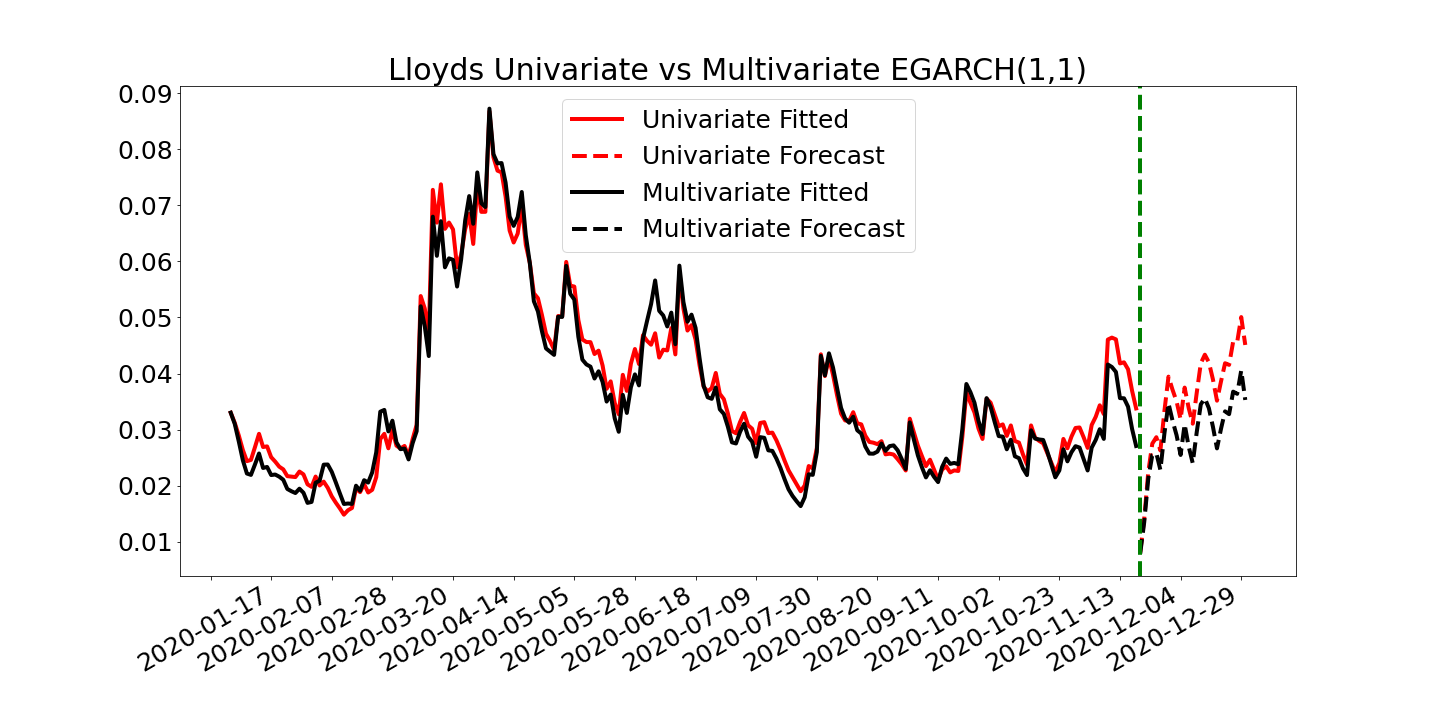
\includegraphics[width=\linewidth]{images/multiGarch/plot 1.png}
  \caption{LLOY}
  \label{fig:A}
\end{subfigure} % <-- "\hfill"
\begin{subfigure}{.49\linewidth}
  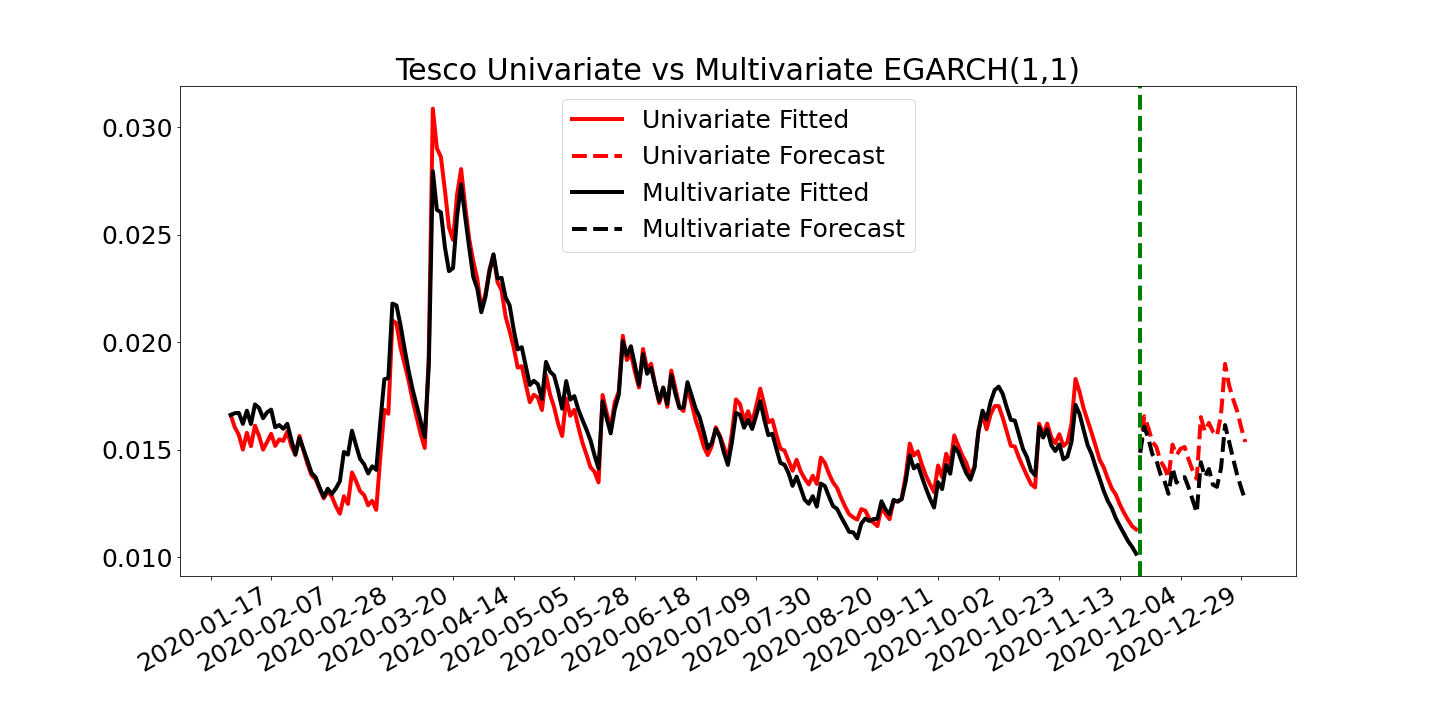
\includegraphics[width=\linewidth]{images/multiGarch/plot 2.png}
  \caption{TSCO}
  \label{fig:B}
\end{subfigure}
\medskip % create some *vertical* separation between the graphs
\begin{subfigure}{.49\linewidth}
  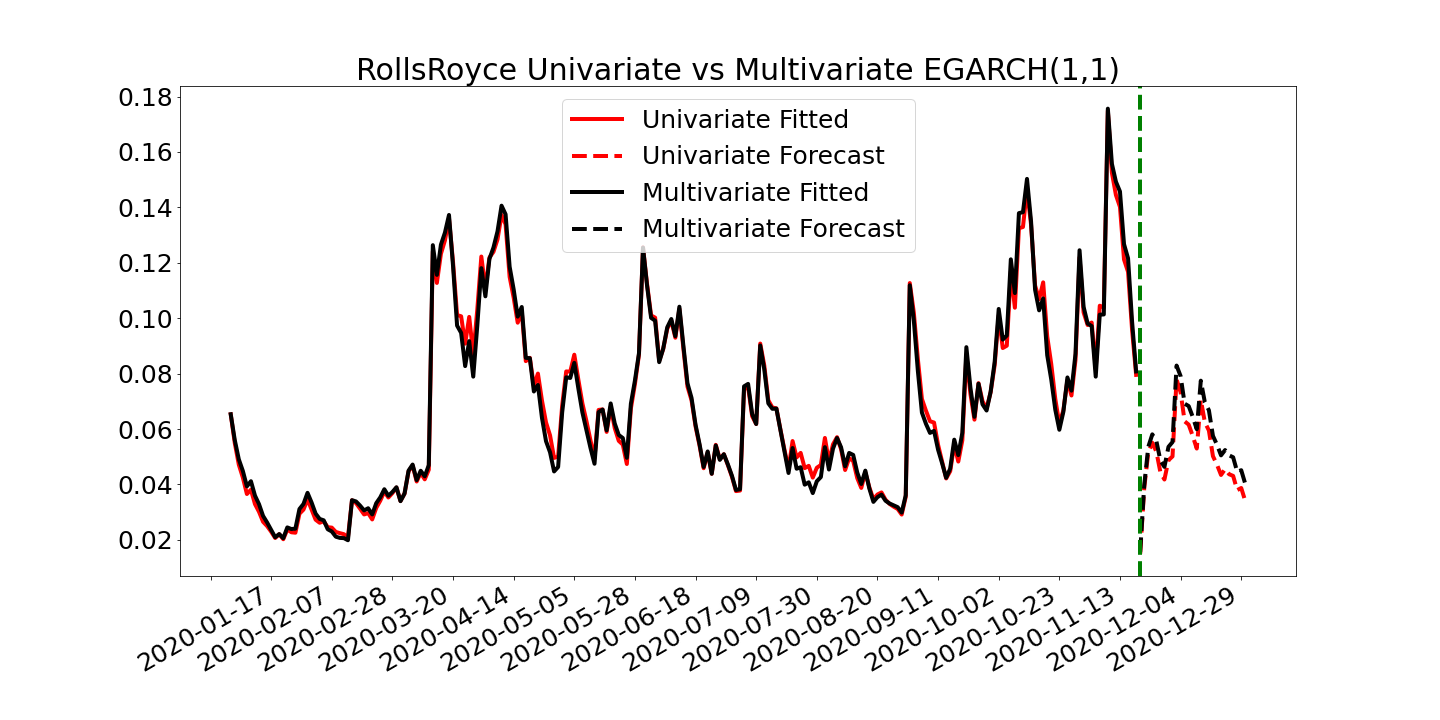
\includegraphics[width=\linewidth]{images/multiGarch/plot 3.png}
  \caption{RR}
  \label{fig:C}
\end{subfigure} % <-- "\hfill"
\begin{subfigure}{.49\linewidth}
  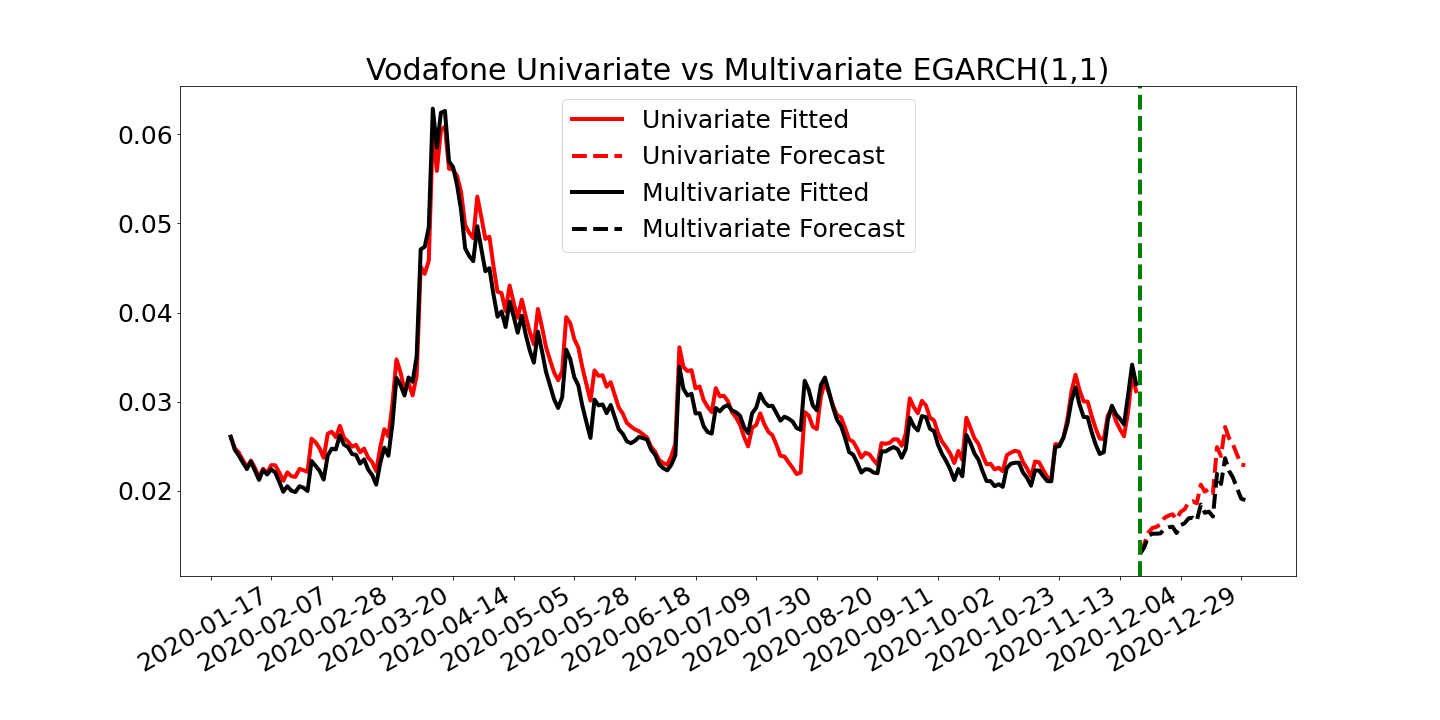
\includegraphics[width=\linewidth]{images/multiGarch/plot 4.png}
  \caption{VOD}
  \label{fig:D}
\end{subfigure}
\caption{Univariate vs Exogenous Forecasts}
\end{figure}

The intuitive interpretation of these results, is the Irithmics short probabilities, when incorporating into the volatility forecast acted almost exclusively as noise rather than signal of the data generating process. Looking closer at the fitted and forecast plots in \textbf{Figure (5.5)}, there are different intensities of impact the exogenous data has on the fitted and forecast values. Sub-figures b and d seem to show more extreme peaks and valleys in the univariate data vs the data incorporating the exogenous data, where sub-figures a and c track the univariate model near identically.